\documentclass[a4paper,12pt]{article}
\usepackage{amsmath, amssymb}
\usepackage{geometry}
\usepackage{enumitem}
\usepackage{fancyhdr}
\usepackage{xcolor}
\usepackage{sectsty}
\usepackage{multicol}
\usepackage{graphicx}
\usepackage{float}
\def\inputGnumericTable{}
\usepackage[latin1]{inputenc}
\usepackage{fullpage}
\usepackage{color}
\usepackage{array}
\usepackage{longtable}
\usepackage{calc}
\usepackage{multirow}
\usepackage{hhline}
\usepackage{ifthen}

\geometry{top=1in, bottom=1.5cm, left=1.5cm, right=1.5cm}

\pagestyle{empty}
\sectionfont{\color{blue}}

\begin{document}

\thispagestyle{fancy}
\fancyhf{}

\fancyhead[L]{

\includegraphics[width=8cm, height=1.7cm]{logo1.jpg}
}

\fancyhead[R]{
Name: Likith Varma \\
Batch: COMETFWC048 \\
Date: March 4th, 2026
}

\renewcommand{\headrulewidth}{0pt}
\fancyfoot[C]{\thepage}

\vspace*{1cm}

\begin{center}
{\LARGE \textbf{\textcolor{blue}{GATE 2009 EE, Question 13 Analysis}}}
\end{center}

\section*{\textbf{Question 13}}

The complete set of only those logic gates designated as Universal Gates is:

\begin{itemize}
\item (A) NOT, OR and AND Gates
\item (B) XNOR, NOR and NAND Gates
\item (C) NOR and NAND Gates
\item (D) XOR, NOR and NAND Gates
\end{itemize}

\section*{\textbf{Question Analysis}}

\begin{itemize}
\item Universal gates are those gates using which any logic circuit can be implemented.
\item NAND gate and NOR gate are called Universal Gates.
\item Both NAND and NOR gates can implement NOT, AND and OR operations.
\item Therefore the correct answer is:
\end{itemize}

\begin{center}
\textbf{Option (C) NOR and NAND Gates}
\end{center}

\newpage

\section*{\textbf{Truth Table}}

\begin{center}

\begin{table}[H]
\centering
\begin{tabular}{|c|c|c|c|}
\hline
A & B & NAND & NOR \\ \hline
0 & 0 & 1 & 1 \\ \hline
0 & 1 & 1 & 0 \\ \hline
1 & 0 & 1 & 0 \\ \hline
1 & 1 & 0 & 0 \\ \hline
\end{tabular}

\end{table}

\end{center}

\section*{\textbf{Hardware Implementation}}

The above logic gates are implemented and tested using an Arduino UNO board and a 7-segment display. Push buttons are used as inputs and the output of the logic gate is displayed on the 7-segment display.

\section*{Required Components \& Pin Connections}

\begin{center}

\begin{minipage}{0.45\textwidth}

\begin{table}[H]
\centering

\begin{tabular}{|c|l|}
\hline
\textbf{S.No} & \textbf{Component} \\ \hline
1 & Arduino UNO Board \\ \hline
2 & Breadboard \\ \hline
3 & 7 Segment Display \\ \hline
4 & Push Buttons (2) \\ \hline
5 & Resistors 220$\Omega$ \\ \hline
6 & Jumper Wires \\ \hline
7 & USB Cable \\ \hline
\end{tabular}

\end{table}

\end{minipage}
\hspace{0.05\textwidth}

\begin{minipage}{0.45\textwidth}

\begin{table}[H]
\centering

\begin{tabular}{|c|c|}
\hline
\textbf{Component} & \textbf{Arduino Pin} \\ \hline
Input P1 & Digital 2 \\ \hline
Input P2 & Digital 3 \\ \hline
Segment a & Digital 4 \\ \hline
Segment b & Digital 5 \\ \hline
Segment c & Digital 6 \\ \hline
Segment d & Digital 7 \\ \hline
Segment e & Digital 8 \\ \hline
Segment f & Digital 9 \\ \hline
Segment g & Digital 10 \\ \hline
GND & GND \\ \hline
VCC & 5V \\ \hline
\end{tabular}

\end{table}

\end{minipage}

\end{center}

\section*{Logic Description}

\begin{itemize}

\item Two push buttons are used as inputs P1 and P2.
\item When buttons are pressed they represent logic value 1.
\item When buttons are not pressed they represent logic value 0.

\item NAND Logic:

\[
Y = \overline{A \cdot B}
\]

\item NOR Logic:

\[
Y = \overline{A + B}
\]

\item The output of the logic gate is displayed on the 7 segment display as either 0 or 1.

\end{itemize}

\section*{Code Uploading Steps}

\begin{enumerate}

\item Create a project folder and write Makefile
\item Write the program in main.c
\item Run command ``make'' to compile the code
\item A .hex file will be generated
\item Copy the .hex file into ArduinoDroid folder
\item Connect Arduino UNO to mobile using OTG cable
\item Upload the file using ``Upload Precompiled'' option
\item Observe the output on the 7-segment display

\end{enumerate}

\section*{Experimental Truth Table}

\begin{table}[H]

\centering

\begin{tabular}{|c|c|c|c|}
\hline
P1 & P2 & NAND Output & NOR Output \\ \hline
0 & 0 & 1 & 1 \\ \hline
0 & 1 & 1 & 0 \\ \hline
1 & 0 & 1 & 0 \\ \hline
1 & 1 & 0 & 0 \\ \hline

\end{tabular}

\end{table}

\begin{center}

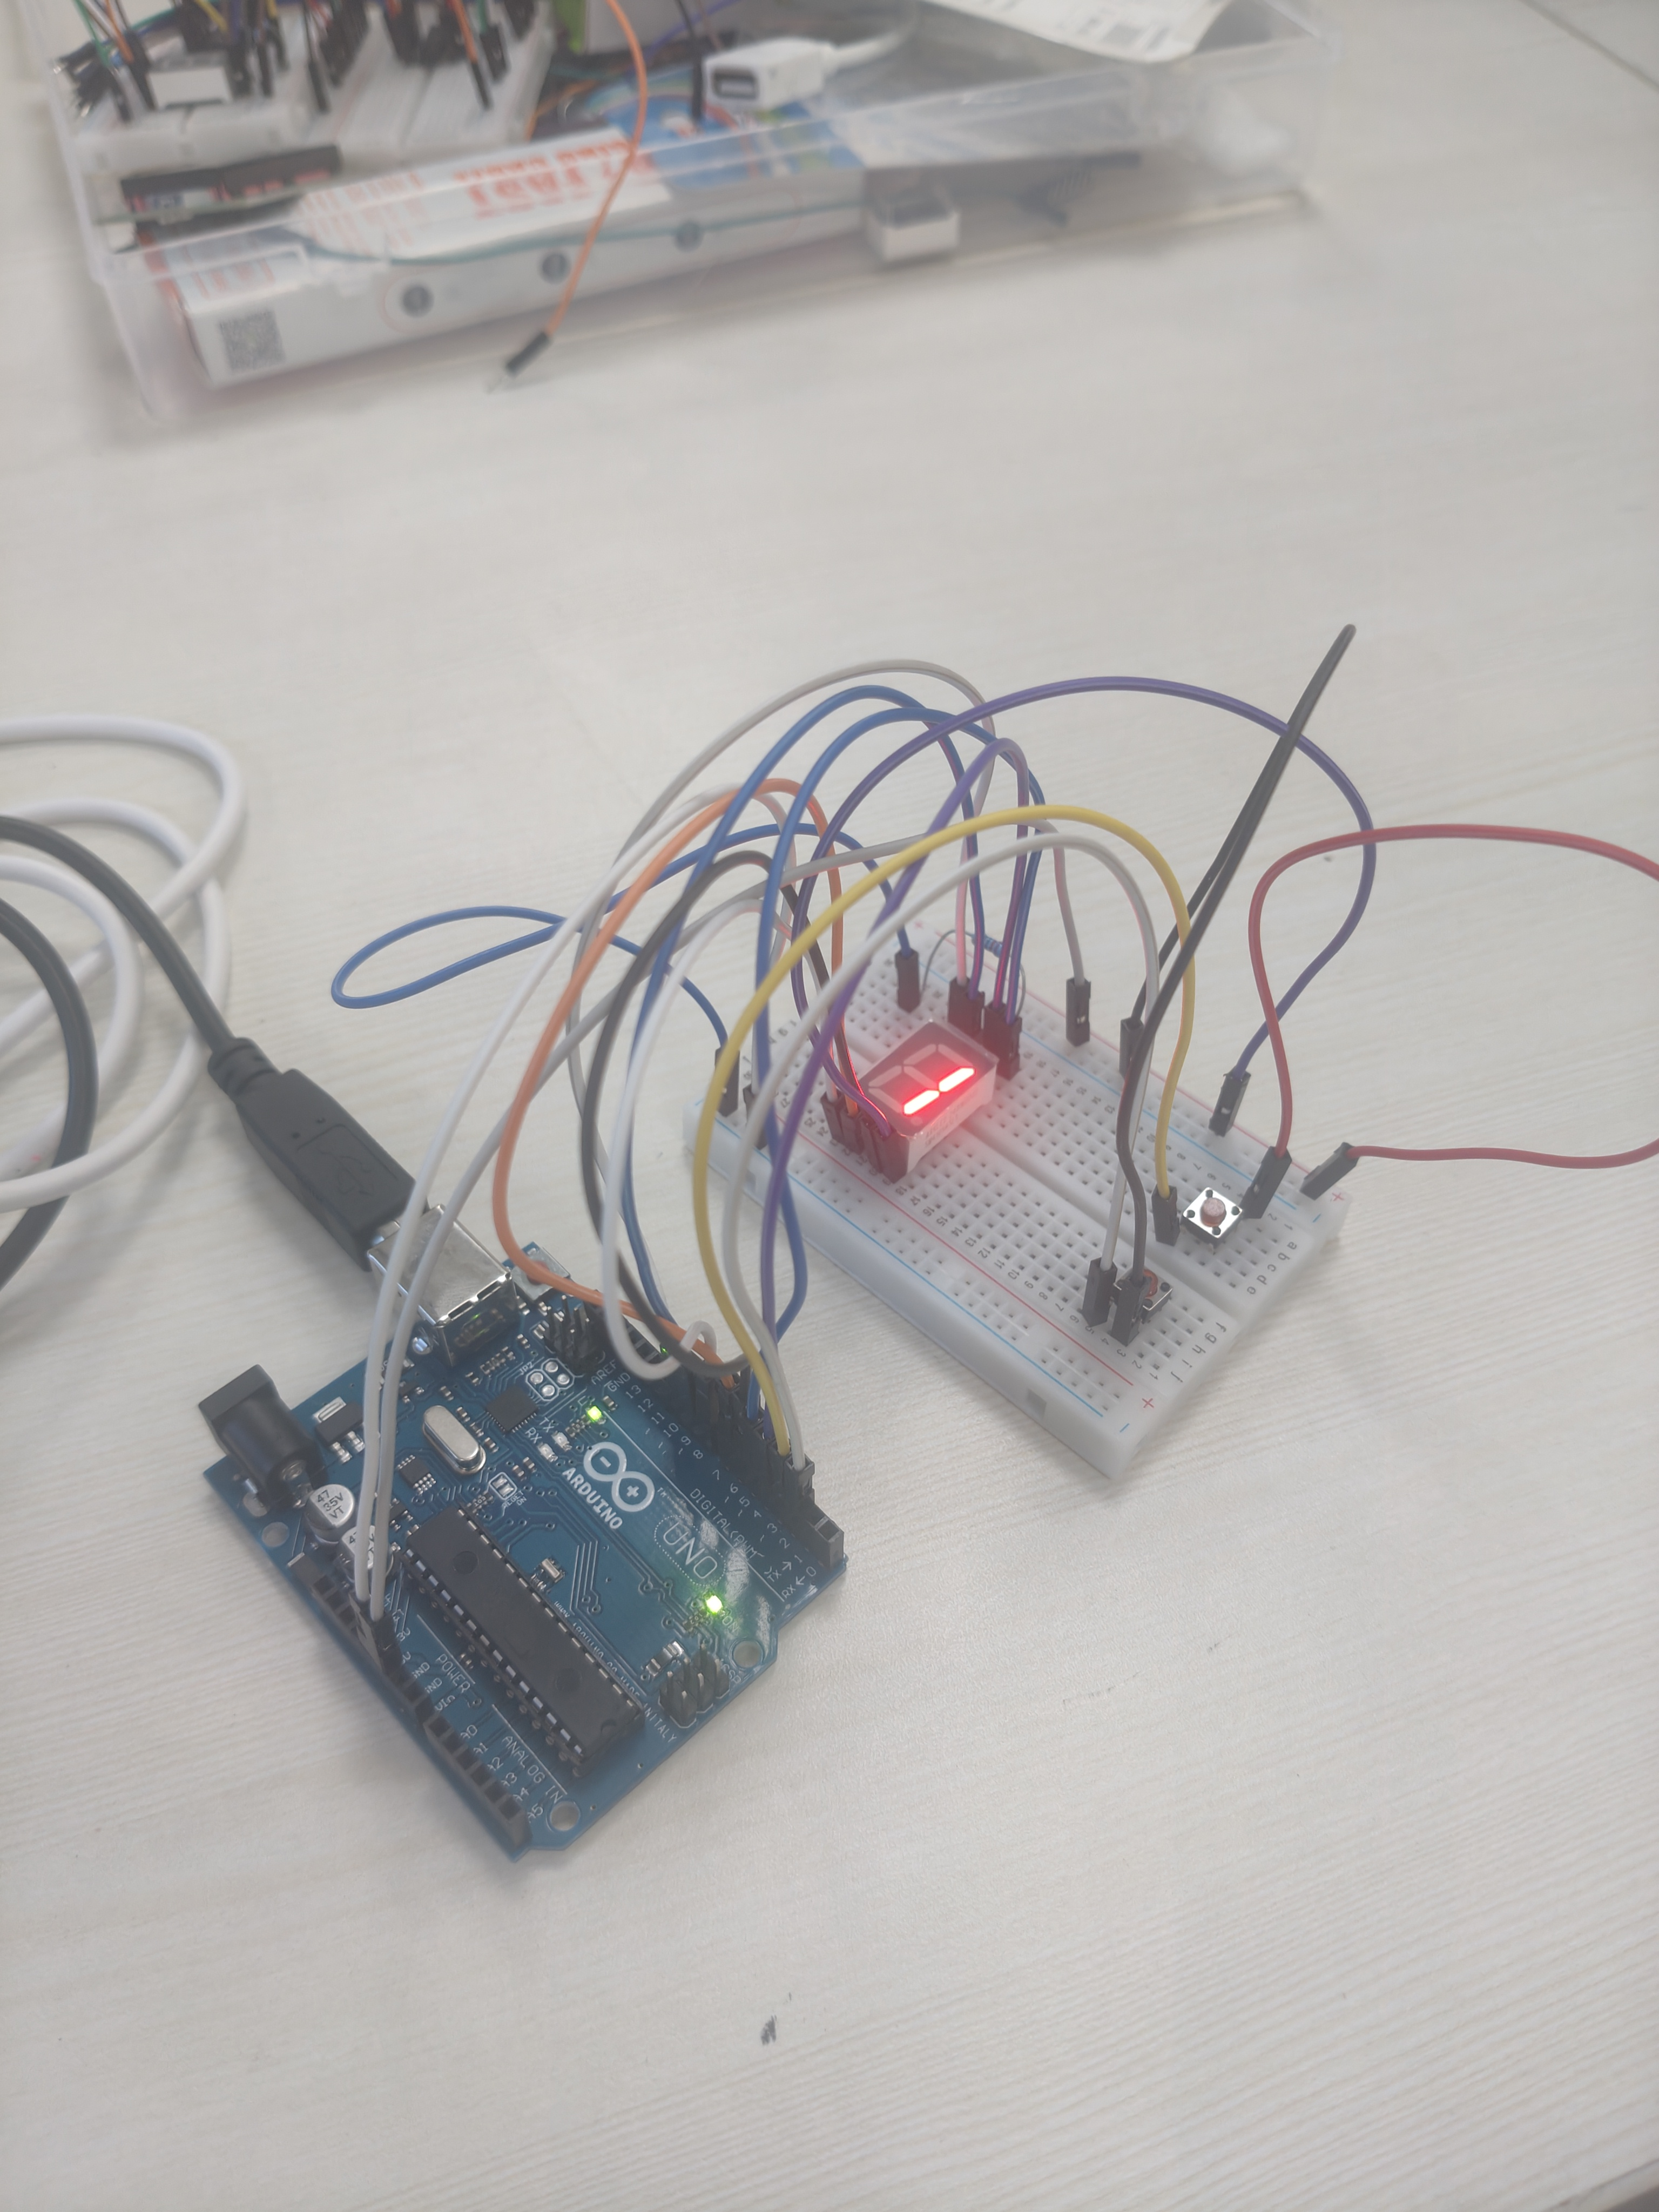
\includegraphics[width=7cm]{output1.jpg}
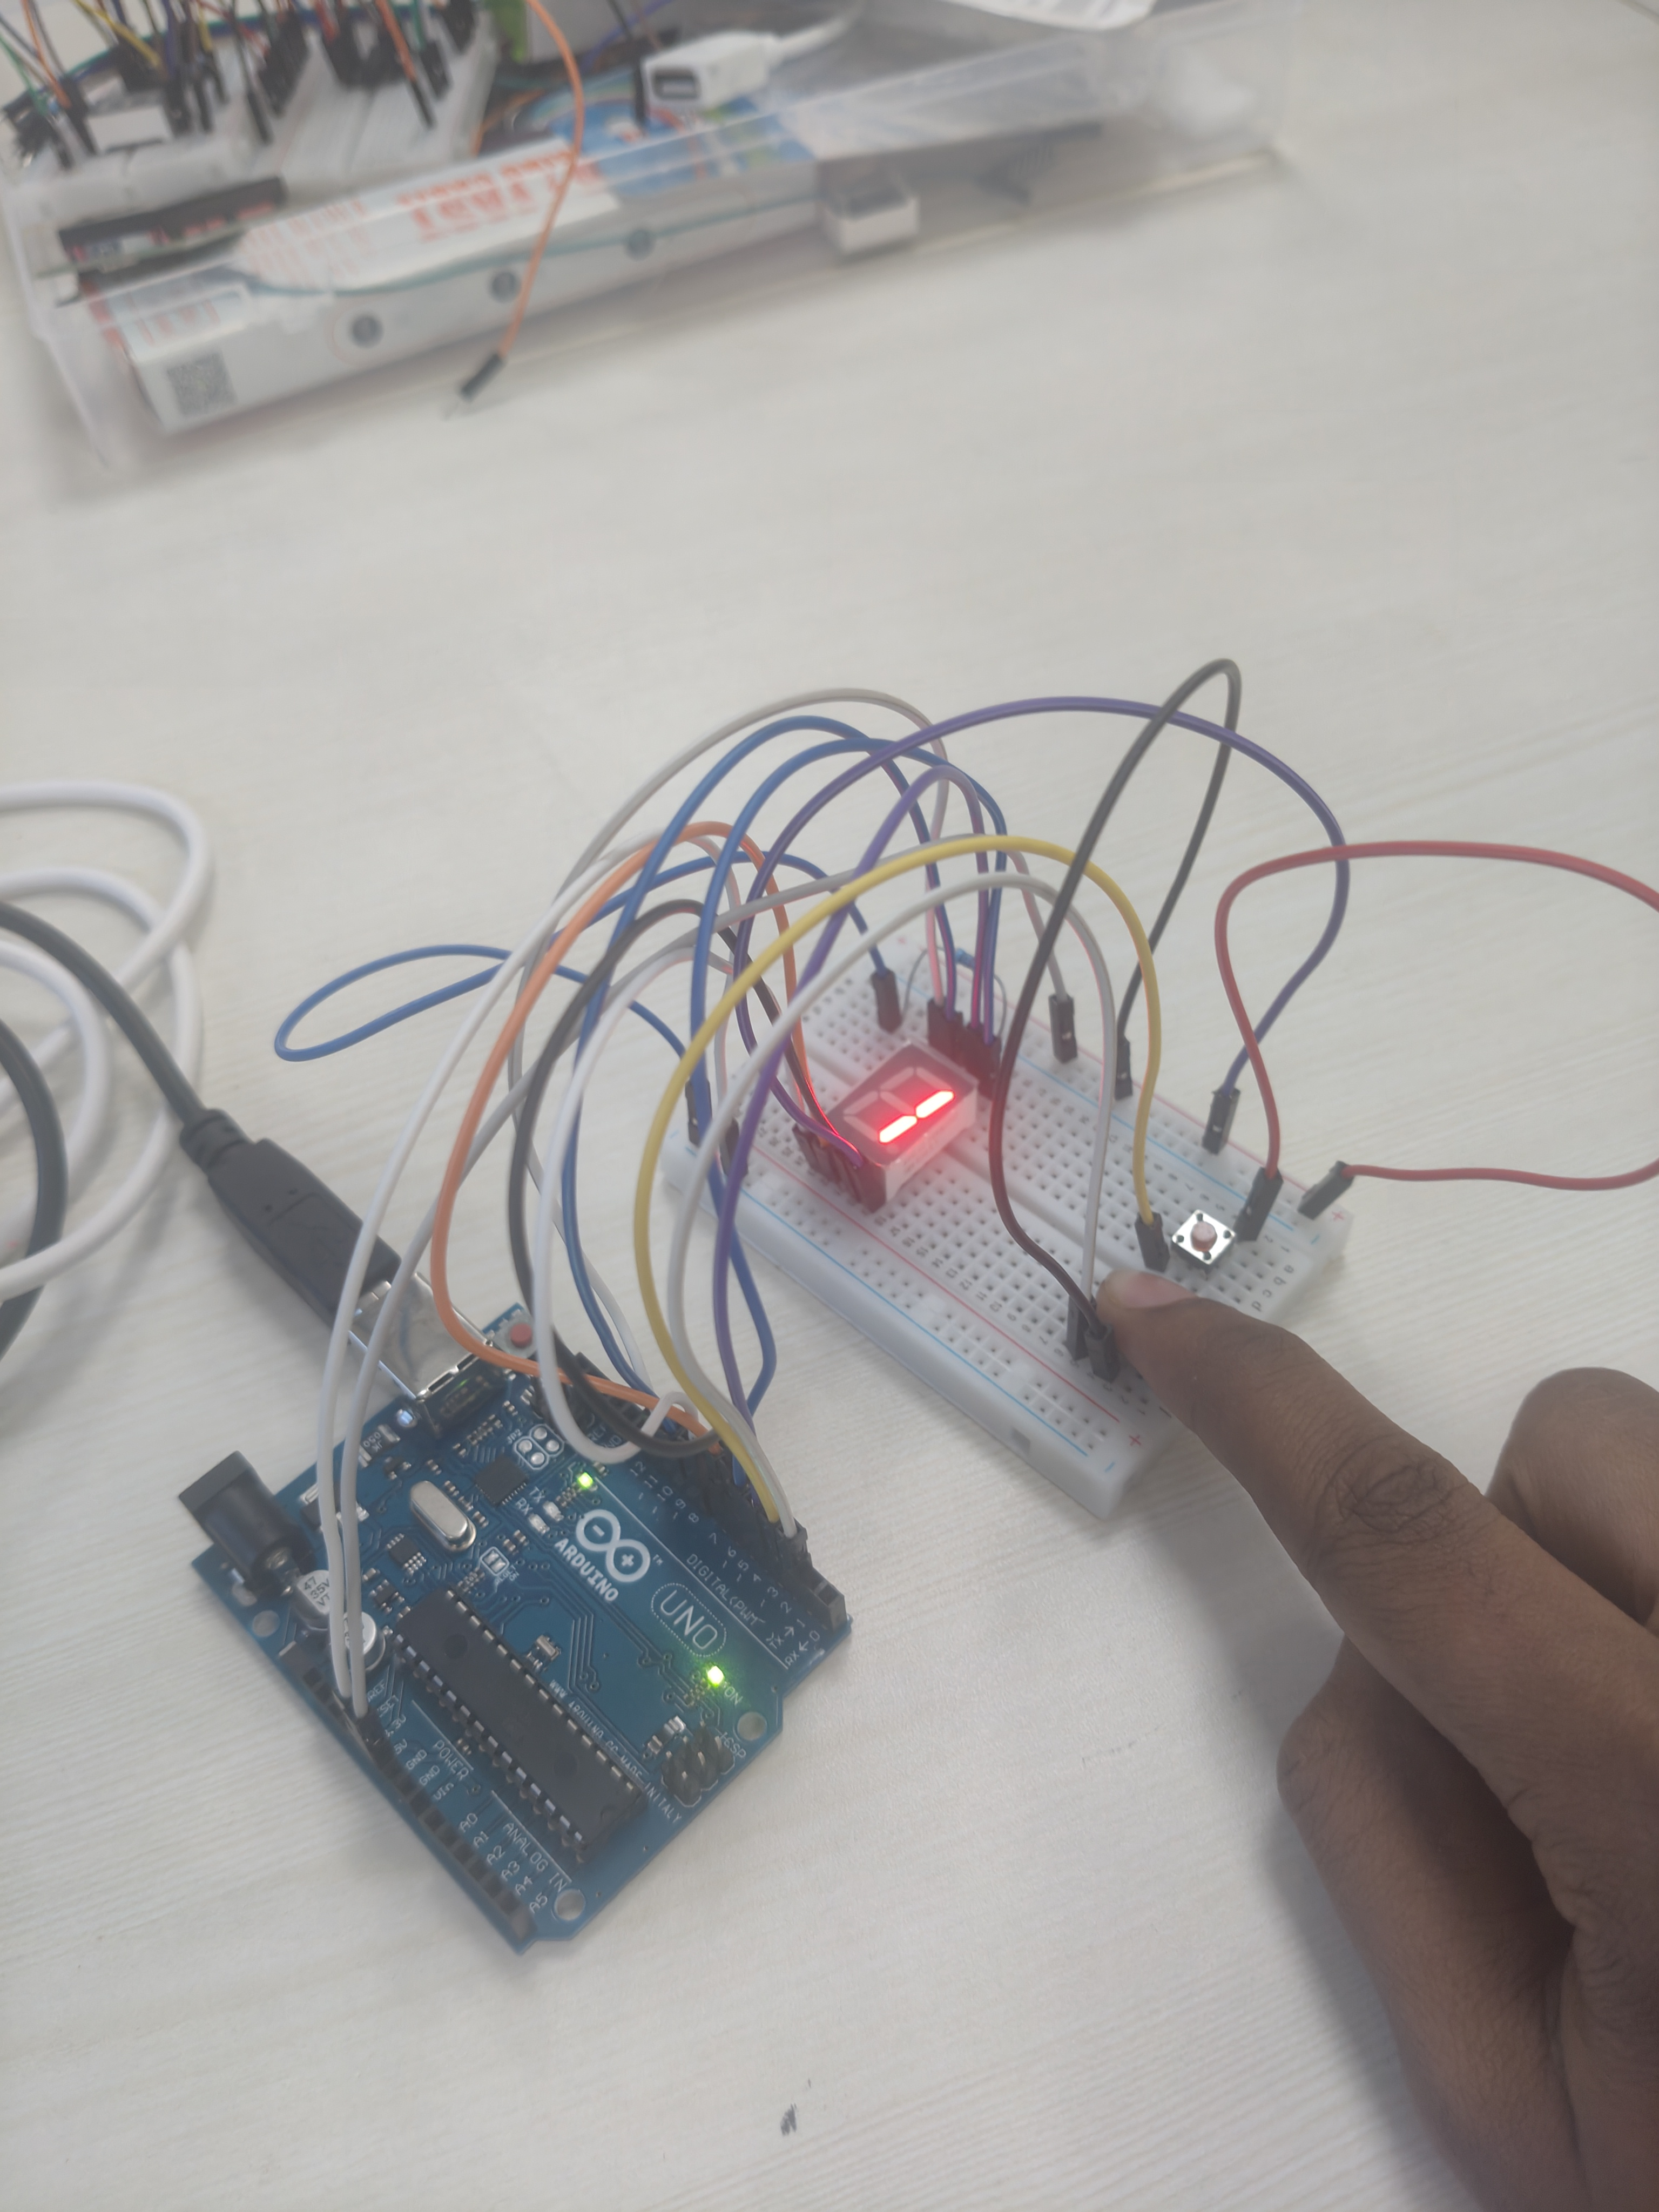
\includegraphics[width=7cm]{output2.jpg}
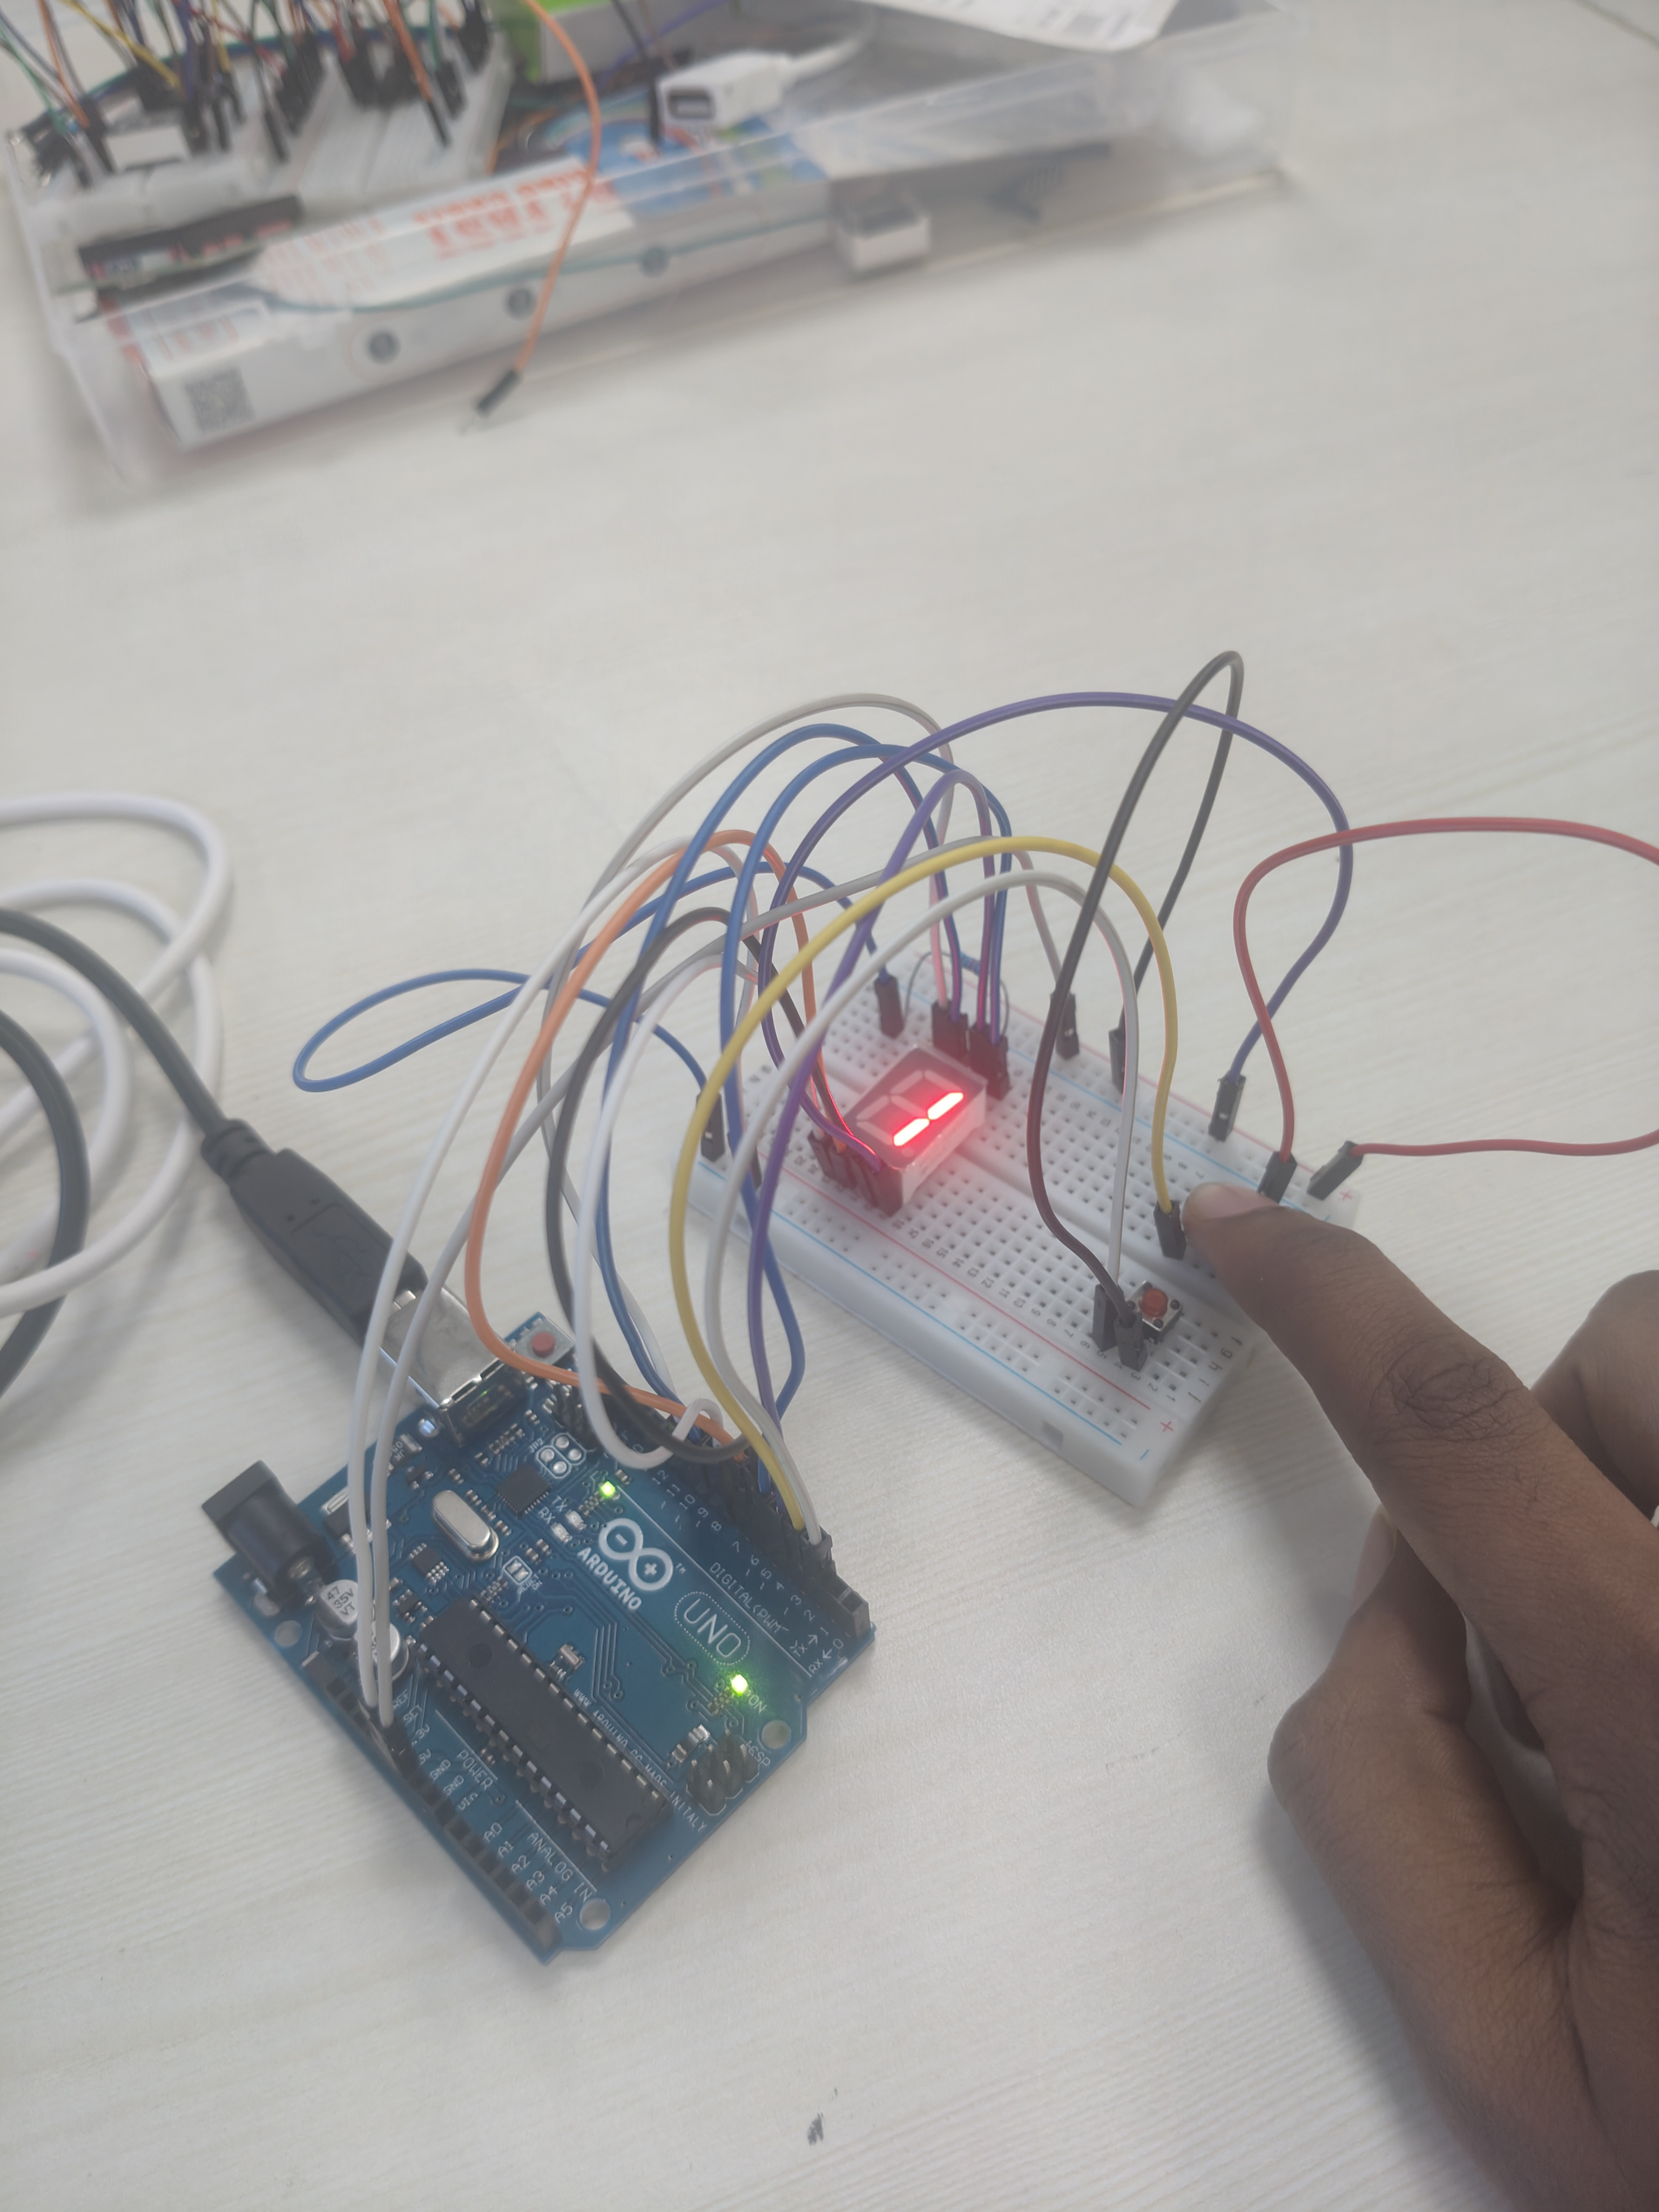
\includegraphics[width=7cm]{output3.jpg}
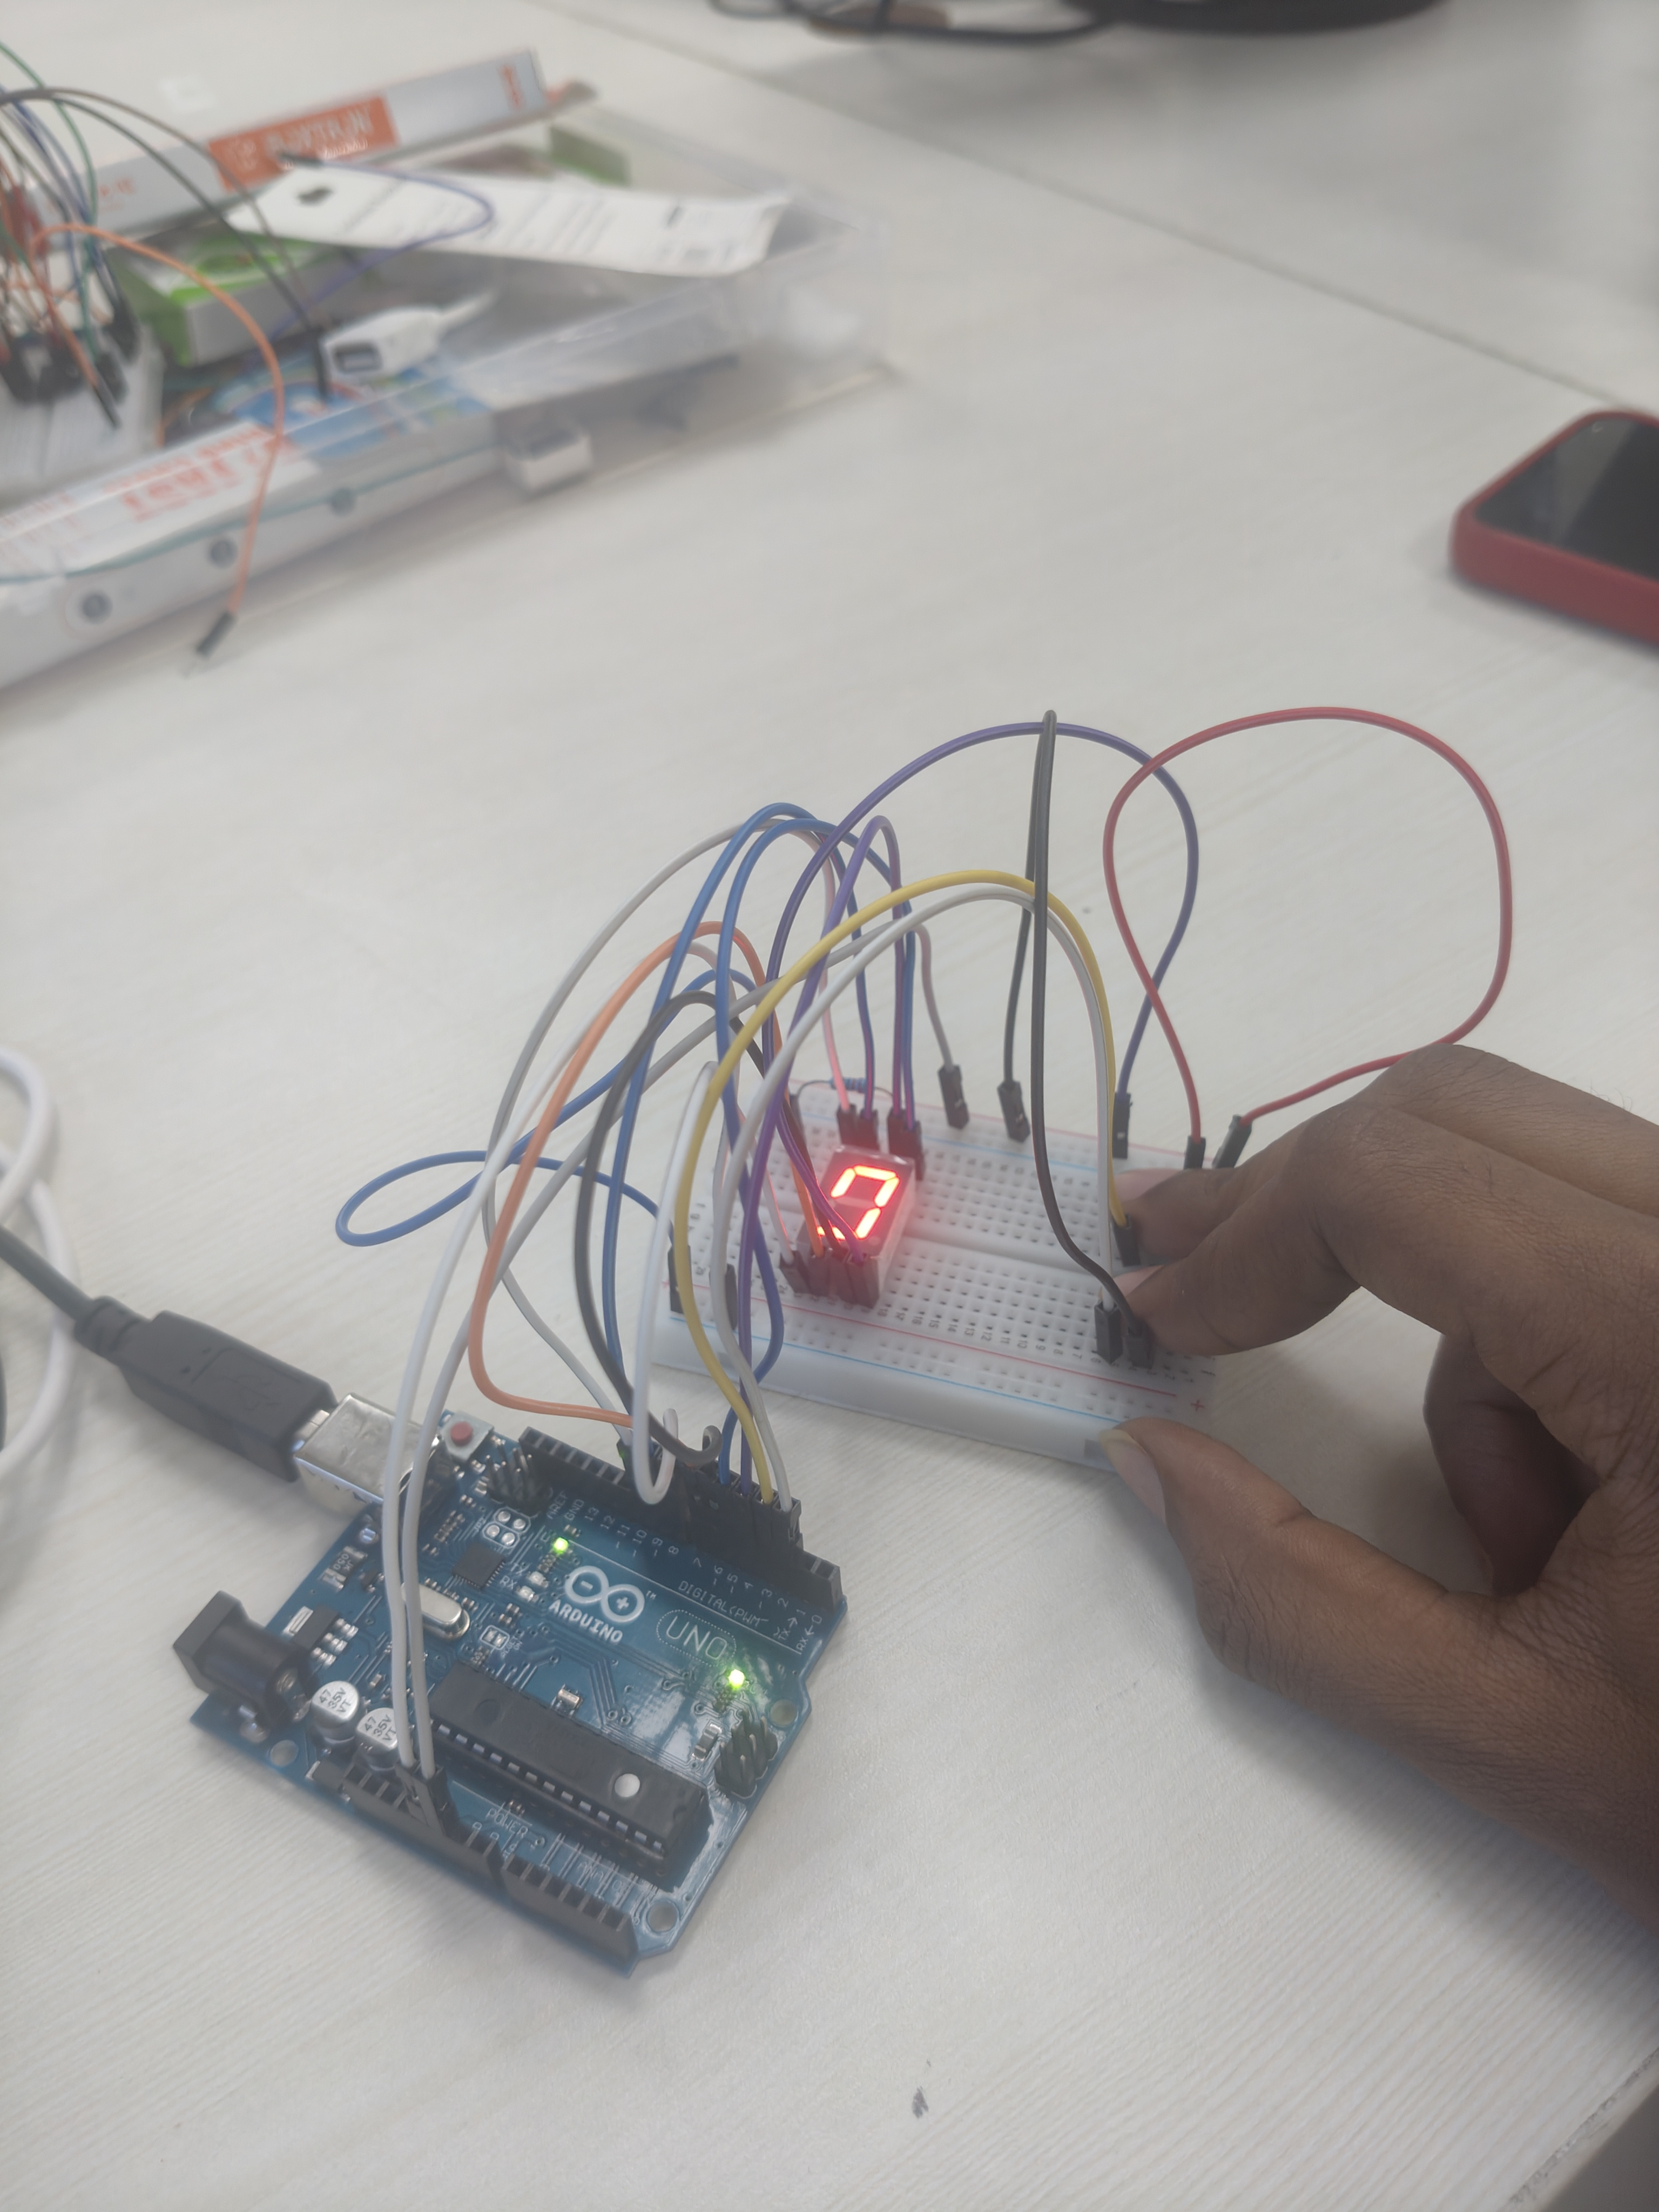
\includegraphics[width=7cm]{output4.jpg}

\end{center}

\section*{Conclusion}

\begin{itemize}

\item NAND and NOR gates are Universal Gates.
\item Using these gates any digital logic circuit can be implemented.
\item Experimental results match the theoretical truth table.
\item Hence the correct answer to GATE 2009 EE Question 13 is Option (C).

\end{itemize}

\end{document}
